\documentclass[twoside]{book}

% Packages required by doxygen
\usepackage{fixltx2e}
\usepackage{calc}
\usepackage{doxygen}
\usepackage[export]{adjustbox} % also loads graphicx
\usepackage{graphicx}
\usepackage[utf8]{inputenc}
\usepackage{makeidx}
\usepackage{multicol}
\usepackage{multirow}
\PassOptionsToPackage{warn}{textcomp}
\usepackage{textcomp}
\usepackage[nointegrals]{wasysym}
\usepackage[table]{xcolor}

% Font selection
\usepackage[T1]{fontenc}
\usepackage[scaled=.90]{helvet}
\usepackage{courier}
\usepackage{amssymb}
\usepackage{sectsty}
\renewcommand{\familydefault}{\sfdefault}
\allsectionsfont{%
  \fontseries{bc}\selectfont%
  \color{darkgray}%
}
\renewcommand{\DoxyLabelFont}{%
  \fontseries{bc}\selectfont%
  \color{darkgray}%
}
\newcommand{\+}{\discretionary{\mbox{\scriptsize$\hookleftarrow$}}{}{}}

% Page & text layout
\usepackage{geometry}
\geometry{%
  a4paper,%
  top=2.5cm,%
  bottom=2.5cm,%
  left=2.5cm,%
  right=2.5cm%
}
\tolerance=750
\hfuzz=15pt
\hbadness=750
\setlength{\emergencystretch}{15pt}
\setlength{\parindent}{0cm}
\setlength{\parskip}{3ex plus 2ex minus 2ex}
\makeatletter
\renewcommand{\paragraph}{%
  \@startsection{paragraph}{4}{0ex}{-1.0ex}{1.0ex}{%
    \normalfont\normalsize\bfseries\SS@parafont%
  }%
}
\renewcommand{\subparagraph}{%
  \@startsection{subparagraph}{5}{0ex}{-1.0ex}{1.0ex}{%
    \normalfont\normalsize\bfseries\SS@subparafont%
  }%
}
\makeatother

% Headers & footers
\usepackage{fancyhdr}
\pagestyle{fancyplain}
\fancyhead[LE]{\fancyplain{}{\bfseries\thepage}}
\fancyhead[CE]{\fancyplain{}{}}
\fancyhead[RE]{\fancyplain{}{\bfseries\leftmark}}
\fancyhead[LO]{\fancyplain{}{\bfseries\rightmark}}
\fancyhead[CO]{\fancyplain{}{}}
\fancyhead[RO]{\fancyplain{}{\bfseries\thepage}}
\fancyfoot[LE]{\fancyplain{}{}}
\fancyfoot[CE]{\fancyplain{}{}}
\fancyfoot[RE]{\fancyplain{}{\bfseries\scriptsize Generated by Doxygen }}
\fancyfoot[LO]{\fancyplain{}{\bfseries\scriptsize Generated by Doxygen }}
\fancyfoot[CO]{\fancyplain{}{}}
\fancyfoot[RO]{\fancyplain{}{}}
\renewcommand{\footrulewidth}{0.4pt}
\renewcommand{\chaptermark}[1]{%
  \markboth{#1}{}%
}
\renewcommand{\sectionmark}[1]{%
  \markright{\thesection\ #1}%
}

% Indices & bibliography
\usepackage{natbib}
\usepackage[titles]{tocloft}
\setcounter{tocdepth}{3}
\setcounter{secnumdepth}{5}
\makeindex

% Hyperlinks (required, but should be loaded last)
\usepackage{ifpdf}
\ifpdf
  \usepackage[pdftex,pagebackref=true]{hyperref}
\else
  \usepackage[ps2pdf,pagebackref=true]{hyperref}
\fi
\hypersetup{%
  colorlinks=true,%
  linkcolor=blue,%
  citecolor=blue,%
  unicode%
}

% Custom commands
\newcommand{\clearemptydoublepage}{%
  \newpage{\pagestyle{empty}\cleardoublepage}%
}

\usepackage{caption}
\captionsetup{labelsep=space,justification=centering,font={bf},singlelinecheck=off,skip=4pt,position=top}

%===== C O N T E N T S =====

\begin{document}

% Titlepage & ToC
\hypersetup{pageanchor=false,
             bookmarksnumbered=true,
             pdfencoding=unicode
            }
\pagenumbering{roman}
\begin{titlepage}
\vspace*{7cm}
\begin{center}%
{\Large My Project }\\
\vspace*{1cm}
{\large Generated by Doxygen 1.8.11}\\
\end{center}
\end{titlepage}
\clearemptydoublepage
\tableofcontents
\clearemptydoublepage
\pagenumbering{arabic}
\hypersetup{pageanchor=true}

%--- Begin generated contents ---
\chapter{File Index}
\section{File List}
Here is a list of all files with brief descriptions\+:\begin{DoxyCompactList}
\item\contentsline{section}{\hyperlink{Lab1_8c}{Lab1.\+c} }{\pageref{Lab1_8c}}{}
\end{DoxyCompactList}

\chapter{File Documentation}
\hypertarget{Stacks_8c}{}\section{Stacks.\+c File Reference}
\label{Stacks_8c}\index{Stacks.\+c@{Stacks.\+c}}
{\ttfamily \#include $<$stdio.\+h$>$}\\*
Include dependency graph for Stacks.\+c\+:
\nopagebreak
\begin{figure}[H]
\begin{center}
\leavevmode
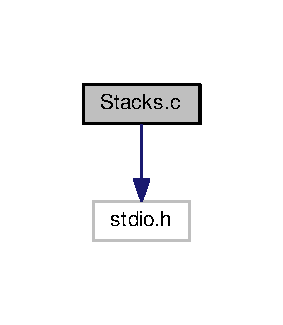
\includegraphics[width=136pt]{Stacks_8c__incl}
\end{center}
\end{figure}
\subsection*{Macros}
\begin{DoxyCompactItemize}
\item 
\#define \hyperlink{Stacks_8c_a70ed59adcb4159ac551058053e649640}{S\+I\+ZE}~10
\end{DoxyCompactItemize}
\subsection*{Functions}
\begin{DoxyCompactItemize}
\item 
void \hyperlink{Stacks_8c_abf1a63ad207c0660c12b37e83b3c90a5}{push\+\_\+stack1} (int data)
\item 
void \hyperlink{Stacks_8c_a8736604ab2d019f3a10c9a5fddf943ea}{push\+\_\+stack2} (int data)
\item 
void \hyperlink{Stacks_8c_a62a6e7a73866ceb9b1394420f9ae17ed}{pop\+\_\+stack1} ()
\item 
void \hyperlink{Stacks_8c_ac64f96854fe1d9851d2ceb24cda6f1dc}{pop\+\_\+stack2} ()
\item 
void \hyperlink{Stacks_8c_a2b6de23813630475797d1a50fa7c25f6}{print\+\_\+stack1} ()
\item 
void \hyperlink{Stacks_8c_ab1b5d48df26cd7605a4daa8e04f77686}{print\+\_\+stack2} ()
\item 
int \hyperlink{Stacks_8c_ae66f6b31b5ad750f1fe042a706a4e3d4}{main} ()
\end{DoxyCompactItemize}
\subsection*{Variables}
\begin{DoxyCompactItemize}
\item 
int \hyperlink{Stacks_8c_a64709c04ff8bebd5ed83bb389ccc8d07}{ar} \mbox{[}\hyperlink{Stacks_8c_a70ed59adcb4159ac551058053e649640}{S\+I\+ZE}\mbox{]}
\item 
int \hyperlink{Stacks_8c_ac543ed64bcbef7101ef43f12f13f735f}{top1} = -\/1
\item 
int \hyperlink{Stacks_8c_acfb319df9526038818b29f54f4596269}{top2} = \hyperlink{Stacks_8c_a70ed59adcb4159ac551058053e649640}{S\+I\+ZE}
\end{DoxyCompactItemize}


\subsection{Macro Definition Documentation}
\index{Stacks.\+c@{Stacks.\+c}!S\+I\+ZE@{S\+I\+ZE}}
\index{S\+I\+ZE@{S\+I\+ZE}!Stacks.\+c@{Stacks.\+c}}
\subsubsection[{\texorpdfstring{S\+I\+ZE}{SIZE}}]{\setlength{\rightskip}{0pt plus 5cm}\#define S\+I\+ZE~10}\hypertarget{Stacks_8c_a70ed59adcb4159ac551058053e649640}{}\label{Stacks_8c_a70ed59adcb4159ac551058053e649640}


\subsection{Function Documentation}
\index{Stacks.\+c@{Stacks.\+c}!main@{main}}
\index{main@{main}!Stacks.\+c@{Stacks.\+c}}
\subsubsection[{\texorpdfstring{main()}{main()}}]{\setlength{\rightskip}{0pt plus 5cm}int main (
\begin{DoxyParamCaption}
{}
\end{DoxyParamCaption}
)}\hypertarget{Stacks_8c_ae66f6b31b5ad750f1fe042a706a4e3d4}{}\label{Stacks_8c_ae66f6b31b5ad750f1fe042a706a4e3d4}

\begin{DoxyCode}
81 \{
82   \textcolor{keywordtype}{int} \hyperlink{Stacks_8c_a64709c04ff8bebd5ed83bb389ccc8d07}{ar}[\hyperlink{Stacks_8c_a70ed59adcb4159ac551058053e649640}{SIZE}];
83   \textcolor{keywordtype}{int} i;
84   \textcolor{keywordtype}{int} num\_of\_ele;
85  
86   printf (\textcolor{stringliteral}{"We can push a total of 10 values\(\backslash\)n"});
87  
88   \textcolor{comment}{//Number of elements pushed in stack 1 is 6}
89   \textcolor{comment}{//Number of elements pushed in stack 2 is 4}
90  
91   \textcolor{keywordflow}{for} (i = 1; i <= 6; ++i)
92   \{
93     \hyperlink{Stacks_8c_abf1a63ad207c0660c12b37e83b3c90a5}{push\_stack1} (i);
94     printf (\textcolor{stringliteral}{"Value Pushed in Stack 1 is %d\(\backslash\)n"}, i);
95   \}
96   \textcolor{keywordflow}{for} (i = 1; i <= 4; ++i)
97   \{
98     \hyperlink{Stacks_8c_a8736604ab2d019f3a10c9a5fddf943ea}{push\_stack2} (i);
99     printf (\textcolor{stringliteral}{"Value Pushed in Stack 2 is %d\(\backslash\)n"}, i);
100   \}
101  
102   \textcolor{comment}{//Print Both Stacks}
103   \hyperlink{Stacks_8c_a2b6de23813630475797d1a50fa7c25f6}{print\_stack1} ();
104   \hyperlink{Stacks_8c_ab1b5d48df26cd7605a4daa8e04f77686}{print\_stack2} ();
105  
106   \textcolor{comment}{//Pushing on Stack Full}
107   printf (\textcolor{stringliteral}{"Pushing Value in Stack 1 is %d\(\backslash\)n"}, 11);
108   \hyperlink{Stacks_8c_abf1a63ad207c0660c12b37e83b3c90a5}{push\_stack1} (11);
109  
110   \textcolor{comment}{//Popping All Elements From Stack 1}
111   num\_of\_ele = \hyperlink{Stacks_8c_ac543ed64bcbef7101ef43f12f13f735f}{top1} + 1;
112   \textcolor{keywordflow}{while} (num\_of\_ele)
113   \{
114     \hyperlink{Stacks_8c_a62a6e7a73866ceb9b1394420f9ae17ed}{pop\_stack1} ();
115     --num\_of\_ele;
116   \}
117  
118   \textcolor{comment}{//Trying to Pop From Empty Stack}
119   \hyperlink{Stacks_8c_a62a6e7a73866ceb9b1394420f9ae17ed}{pop\_stack1} ();
120  
121   \textcolor{keywordflow}{return} 0;
122 \}\end{DoxyCode}


Here is the call graph for this function\+:
\nopagebreak
\begin{figure}[H]
\begin{center}
\leavevmode
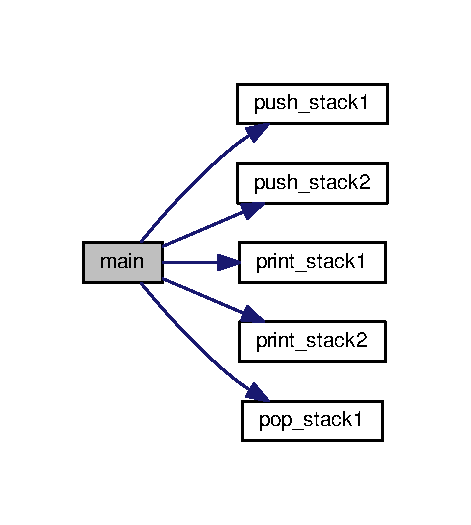
\includegraphics[width=226pt]{Stacks_8c_ae66f6b31b5ad750f1fe042a706a4e3d4_cgraph}
\end{center}
\end{figure}


\index{Stacks.\+c@{Stacks.\+c}!pop\+\_\+stack1@{pop\+\_\+stack1}}
\index{pop\+\_\+stack1@{pop\+\_\+stack1}!Stacks.\+c@{Stacks.\+c}}
\subsubsection[{\texorpdfstring{pop\+\_\+stack1()}{pop_stack1()}}]{\setlength{\rightskip}{0pt plus 5cm}void pop\+\_\+stack1 (
\begin{DoxyParamCaption}
{}
\end{DoxyParamCaption}
)}\hypertarget{Stacks_8c_a62a6e7a73866ceb9b1394420f9ae17ed}{}\label{Stacks_8c_a62a6e7a73866ceb9b1394420f9ae17ed}

\begin{DoxyCode}
36 \{
37   \textcolor{keywordflow}{if} (\hyperlink{Stacks_8c_ac543ed64bcbef7101ef43f12f13f735f}{top1} >= 0)
38   \{
39     \textcolor{keywordtype}{int} popped\_value = \hyperlink{Stacks_8c_a64709c04ff8bebd5ed83bb389ccc8d07}{ar}[\hyperlink{Stacks_8c_ac543ed64bcbef7101ef43f12f13f735f}{top1}--];
40     printf (\textcolor{stringliteral}{"%d is being popped from Stack 1\(\backslash\)n"}, popped\_value);
41   \}
42   \textcolor{keywordflow}{else}
43   \{
44     printf (\textcolor{stringliteral}{"Stack Empty! Cannot Pop\(\backslash\)n"});
45   \}
46 \}
\end{DoxyCode}
\index{Stacks.\+c@{Stacks.\+c}!pop\+\_\+stack2@{pop\+\_\+stack2}}
\index{pop\+\_\+stack2@{pop\+\_\+stack2}!Stacks.\+c@{Stacks.\+c}}
\subsubsection[{\texorpdfstring{pop\+\_\+stack2()}{pop_stack2()}}]{\setlength{\rightskip}{0pt plus 5cm}void pop\+\_\+stack2 (
\begin{DoxyParamCaption}
{}
\end{DoxyParamCaption}
)}\hypertarget{Stacks_8c_ac64f96854fe1d9851d2ceb24cda6f1dc}{}\label{Stacks_8c_ac64f96854fe1d9851d2ceb24cda6f1dc}

\begin{DoxyCode}
48 \{
49   \textcolor{keywordflow}{if} (\hyperlink{Stacks_8c_acfb319df9526038818b29f54f4596269}{top2} < \hyperlink{Stacks_8c_a70ed59adcb4159ac551058053e649640}{SIZE})
50   \{
51     \textcolor{keywordtype}{int} popped\_value = \hyperlink{Stacks_8c_a64709c04ff8bebd5ed83bb389ccc8d07}{ar}[\hyperlink{Stacks_8c_acfb319df9526038818b29f54f4596269}{top2}++];
52     printf (\textcolor{stringliteral}{"%d is being popped from Stack 2\(\backslash\)n"}, popped\_value);
53   \}
54   \textcolor{keywordflow}{else}
55   \{
56     printf (\textcolor{stringliteral}{"Stack Empty! Cannot Pop\(\backslash\)n"});
57   \}
58 \}
\end{DoxyCode}
\index{Stacks.\+c@{Stacks.\+c}!print\+\_\+stack1@{print\+\_\+stack1}}
\index{print\+\_\+stack1@{print\+\_\+stack1}!Stacks.\+c@{Stacks.\+c}}
\subsubsection[{\texorpdfstring{print\+\_\+stack1()}{print_stack1()}}]{\setlength{\rightskip}{0pt plus 5cm}void print\+\_\+stack1 (
\begin{DoxyParamCaption}
{}
\end{DoxyParamCaption}
)}\hypertarget{Stacks_8c_a2b6de23813630475797d1a50fa7c25f6}{}\label{Stacks_8c_a2b6de23813630475797d1a50fa7c25f6}

\begin{DoxyCode}
62 \{
63   \textcolor{keywordtype}{int} i;
64   \textcolor{keywordflow}{for} (i = \hyperlink{Stacks_8c_ac543ed64bcbef7101ef43f12f13f735f}{top1}; i >= 0; --i)
65   \{
66     printf (\textcolor{stringliteral}{"%d "}, \hyperlink{Stacks_8c_a64709c04ff8bebd5ed83bb389ccc8d07}{ar}[i]);
67   \}
68   printf (\textcolor{stringliteral}{"\(\backslash\)n"});
69 \}
\end{DoxyCode}
\index{Stacks.\+c@{Stacks.\+c}!print\+\_\+stack2@{print\+\_\+stack2}}
\index{print\+\_\+stack2@{print\+\_\+stack2}!Stacks.\+c@{Stacks.\+c}}
\subsubsection[{\texorpdfstring{print\+\_\+stack2()}{print_stack2()}}]{\setlength{\rightskip}{0pt plus 5cm}void print\+\_\+stack2 (
\begin{DoxyParamCaption}
{}
\end{DoxyParamCaption}
)}\hypertarget{Stacks_8c_ab1b5d48df26cd7605a4daa8e04f77686}{}\label{Stacks_8c_ab1b5d48df26cd7605a4daa8e04f77686}

\begin{DoxyCode}
71 \{
72   \textcolor{keywordtype}{int} i;
73   \textcolor{keywordflow}{for} (i = \hyperlink{Stacks_8c_acfb319df9526038818b29f54f4596269}{top2}; i < \hyperlink{Stacks_8c_a70ed59adcb4159ac551058053e649640}{SIZE}; ++i)
74   \{
75     printf (\textcolor{stringliteral}{"%d "}, \hyperlink{Stacks_8c_a64709c04ff8bebd5ed83bb389ccc8d07}{ar}[i]);
76   \}
77   printf (\textcolor{stringliteral}{"\(\backslash\)n"});
78 \}
\end{DoxyCode}
\index{Stacks.\+c@{Stacks.\+c}!push\+\_\+stack1@{push\+\_\+stack1}}
\index{push\+\_\+stack1@{push\+\_\+stack1}!Stacks.\+c@{Stacks.\+c}}
\subsubsection[{\texorpdfstring{push\+\_\+stack1(int data)}{push_stack1(int data)}}]{\setlength{\rightskip}{0pt plus 5cm}void push\+\_\+stack1 (
\begin{DoxyParamCaption}
\item[{int}]{data}
\end{DoxyParamCaption}
)}\hypertarget{Stacks_8c_abf1a63ad207c0660c12b37e83b3c90a5}{}\label{Stacks_8c_abf1a63ad207c0660c12b37e83b3c90a5}

\begin{DoxyCode}
12 \{
13   \textcolor{keywordflow}{if} (\hyperlink{Stacks_8c_ac543ed64bcbef7101ef43f12f13f735f}{top1} < \hyperlink{Stacks_8c_acfb319df9526038818b29f54f4596269}{top2} - 1)
14   \{
15     \hyperlink{Stacks_8c_a64709c04ff8bebd5ed83bb389ccc8d07}{ar}[++\hyperlink{Stacks_8c_ac543ed64bcbef7101ef43f12f13f735f}{top1}] = data;
16   \}
17   \textcolor{keywordflow}{else}
18   \{
19     printf (\textcolor{stringliteral}{"Stack Full! Cannot Push\(\backslash\)n"});
20   \}
21 \}
\end{DoxyCode}
\index{Stacks.\+c@{Stacks.\+c}!push\+\_\+stack2@{push\+\_\+stack2}}
\index{push\+\_\+stack2@{push\+\_\+stack2}!Stacks.\+c@{Stacks.\+c}}
\subsubsection[{\texorpdfstring{push\+\_\+stack2(int data)}{push_stack2(int data)}}]{\setlength{\rightskip}{0pt plus 5cm}void push\+\_\+stack2 (
\begin{DoxyParamCaption}
\item[{int}]{data}
\end{DoxyParamCaption}
)}\hypertarget{Stacks_8c_a8736604ab2d019f3a10c9a5fddf943ea}{}\label{Stacks_8c_a8736604ab2d019f3a10c9a5fddf943ea}

\begin{DoxyCode}
23 \{
24   \textcolor{keywordflow}{if} (\hyperlink{Stacks_8c_ac543ed64bcbef7101ef43f12f13f735f}{top1} < \hyperlink{Stacks_8c_acfb319df9526038818b29f54f4596269}{top2} - 1)
25   \{
26     \hyperlink{Stacks_8c_a64709c04ff8bebd5ed83bb389ccc8d07}{ar}[--\hyperlink{Stacks_8c_acfb319df9526038818b29f54f4596269}{top2}] = data; 
27   \}
28   \textcolor{keywordflow}{else}
29   \{
30     printf (\textcolor{stringliteral}{"Stack Full! Cannot Push\(\backslash\)n"});
31   \}
32 \}
\end{DoxyCode}


\subsection{Variable Documentation}
\index{Stacks.\+c@{Stacks.\+c}!ar@{ar}}
\index{ar@{ar}!Stacks.\+c@{Stacks.\+c}}
\subsubsection[{\texorpdfstring{ar}{ar}}]{\setlength{\rightskip}{0pt plus 5cm}int ar\mbox{[}{\bf S\+I\+ZE}\mbox{]}}\hypertarget{Stacks_8c_a64709c04ff8bebd5ed83bb389ccc8d07}{}\label{Stacks_8c_a64709c04ff8bebd5ed83bb389ccc8d07}
\index{Stacks.\+c@{Stacks.\+c}!top1@{top1}}
\index{top1@{top1}!Stacks.\+c@{Stacks.\+c}}
\subsubsection[{\texorpdfstring{top1}{top1}}]{\setlength{\rightskip}{0pt plus 5cm}int top1 = -\/1}\hypertarget{Stacks_8c_ac543ed64bcbef7101ef43f12f13f735f}{}\label{Stacks_8c_ac543ed64bcbef7101ef43f12f13f735f}
\index{Stacks.\+c@{Stacks.\+c}!top2@{top2}}
\index{top2@{top2}!Stacks.\+c@{Stacks.\+c}}
\subsubsection[{\texorpdfstring{top2}{top2}}]{\setlength{\rightskip}{0pt plus 5cm}int top2 = {\bf S\+I\+ZE}}\hypertarget{Stacks_8c_acfb319df9526038818b29f54f4596269}{}\label{Stacks_8c_acfb319df9526038818b29f54f4596269}

%--- End generated contents ---

% Index
\backmatter
\newpage
\phantomsection
\clearemptydoublepage
\addcontentsline{toc}{chapter}{Index}
\printindex

\end{document}
